
\section{Experiment Setup} \label{sec:setup}

We design a system using the tools we introduce above including SVEF, bmv2, and P4. Because of the limit of fund, we use bmv2 inside mininet and test our three drop logics. Three scenarios are designed to compare the difference among these drop logics. 

We use real H.264/SVC video sequences in our experiments, and these scenarios are done in mininet with software MANEs (running {\em bmv2}~cite{bmv2}) and virtual hosts.
In these scenarios, we would like to see the characteristic of P4 and our contribution. These three scenarios are described below:

Fig. ~\ref{scenario1}, ~\ref{scenario2} and ~\ref{scenario3} are scenarios we use to evaluate tail and EL logics. The RDO logic will be test only in scenario 3.

\begin{figure}[tbh]
	\centering
	\begin{minipage}[t]{0.24\textwidth}
	\centering
	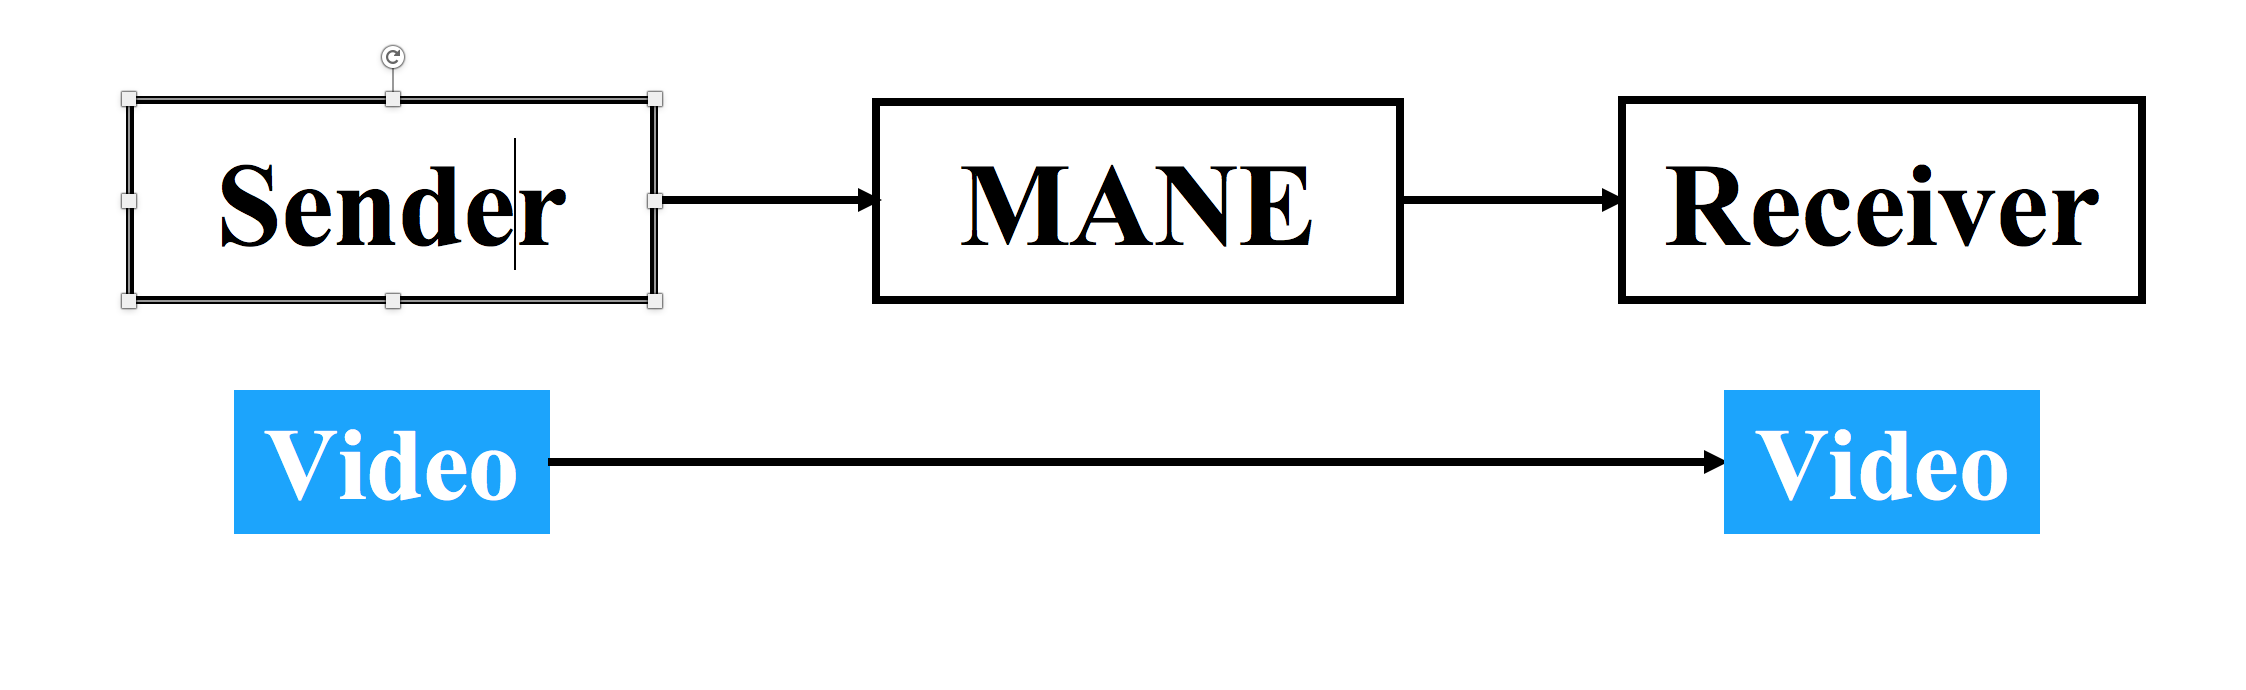
\includegraphics[width=\textwidth]{fig/scenario1.png}
	\caption{Testbed topology (scenarios 1).}
	\label{scenario1} 
	\end{minipage}
	\hfill\begin{minipage}[t]{0.23\textwidth}
	\centering
	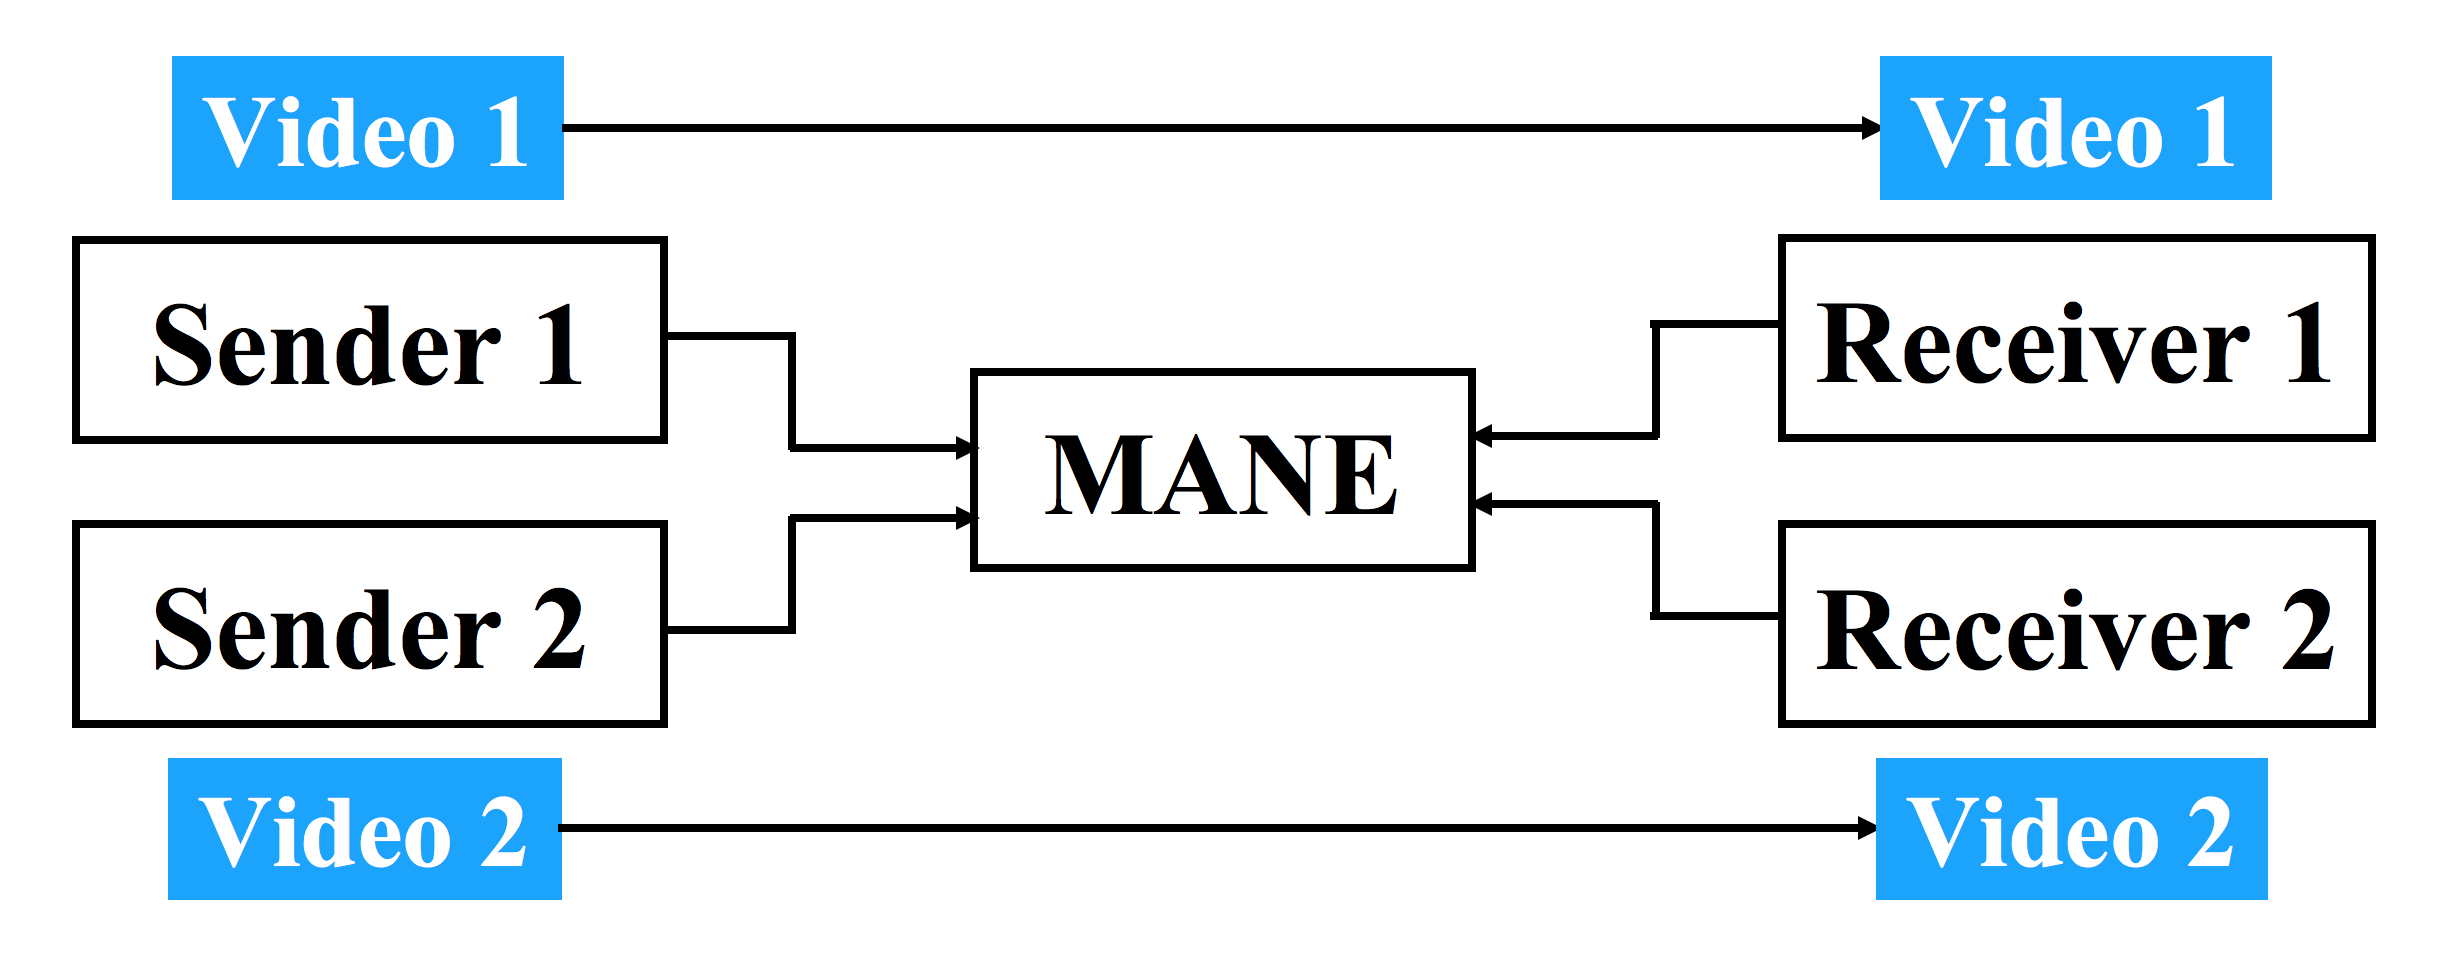
\includegraphics[width=\textwidth]{fig/scenario2.png}
	\caption{Testbed topology (scenario 2).}
	\label{scenario2} 
	\end{minipage}
	\vspace{-0.1cm}
\end{figure}

\begin{itemize} 
	\item {\bf Intelligent packet drops of a single video stream.}
	We construct a simple network with a sender, a controller, a MANE, and a receiver. Scenario 1 is the simplest topology. It consists of one sender and one receiver streaming one video. In this scenario, we want to observe the drawbacks of tail logic and see if EL logic can reduce network congestion by eliminate undecodable packets. The mininet bandwidth on the link is varied over time by scripts. In the MANE, we implement tail, EL, and RDO logics, and compare their performance. 

	\item {\bf Optimal packet drops across multiple video streams.}
	Scenario 2 is has four hosts with two sender and two receiver streaming two videos in mininet. In this scenario, we can use twice of buffer than scenario 1 because packets should be forwarded to different hosts and pushed into different buffer. In the MANE, we also implement three drop logics, and We can imagine that the result of scenario 1 and 2 would be very similar.

	\item{\bf Eliminate undecodable packets in less buffer}
	Scenario 3 shown in Fig.~\ref{scenario3} is the most challenging one. It contains one sender and one receiver streaming two videos in the same time. In this scenario, two streaming flows could affect each other since there is still exist a small time gap between them. When our P4-based MANE receive packets. It could push packets belong to one of the streaming flow but drop the other since the size of buffer exceed threshold after pushing that packet. 

\end{itemize}

\begin{figure}[tbh]
	\centering
	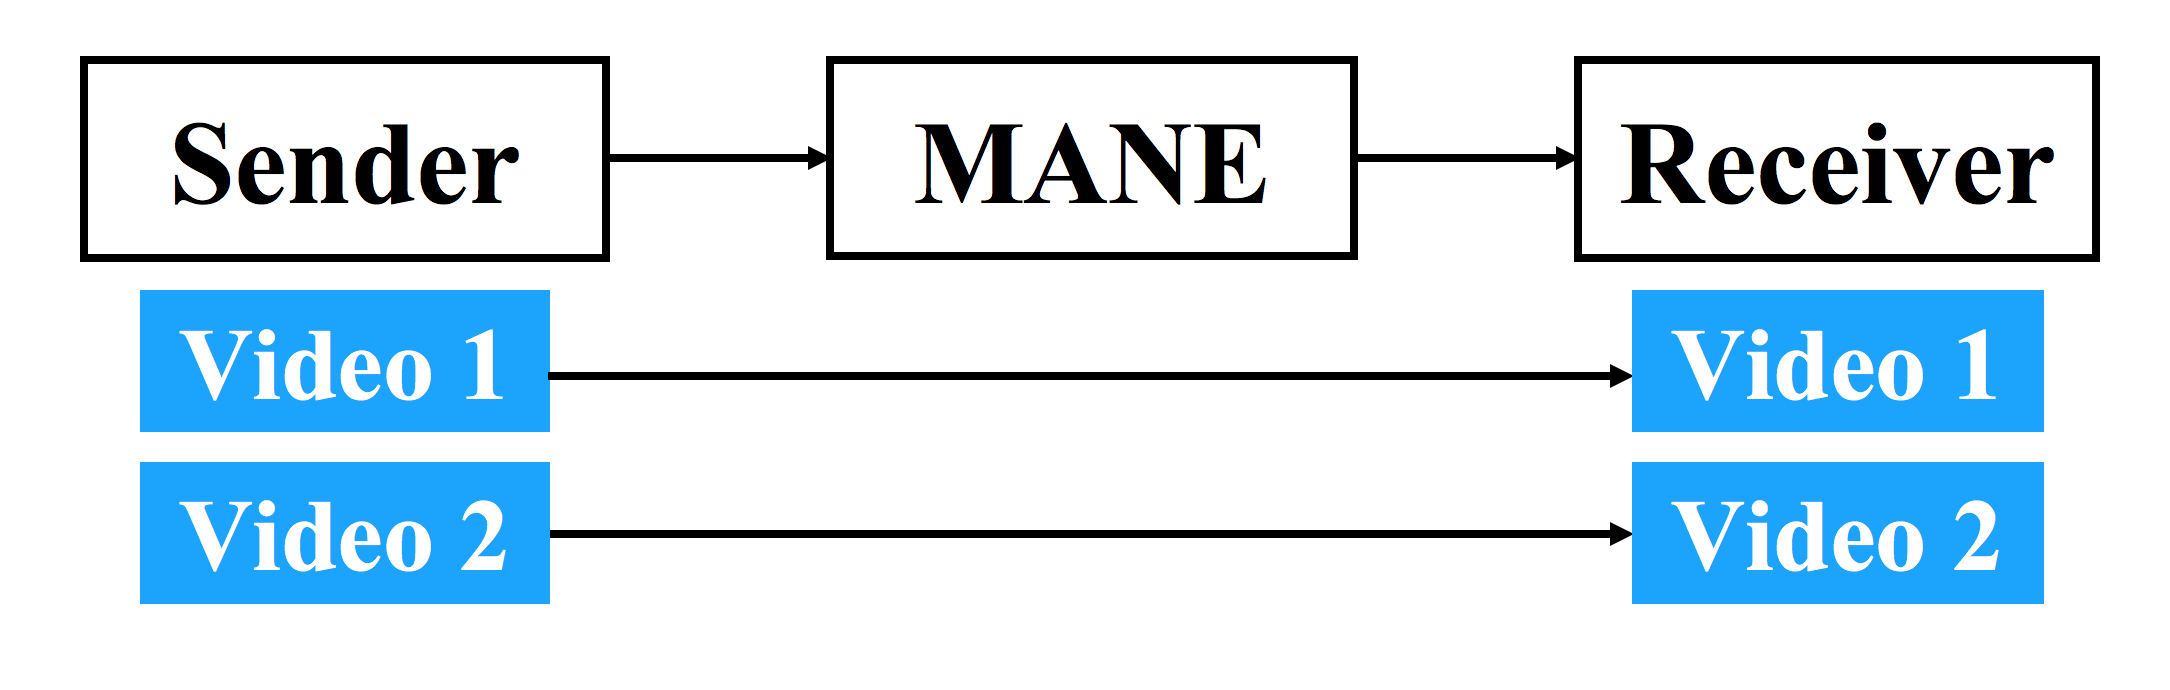
\includegraphics[width=.50\textwidth]{fig/scenario3.png}
	\caption{Testbed topology (scenarios 3).}
	\label{scenario3} 
\end{figure}

Among these scenarios. We try to limit the bandwidth between all of the links using tclink of mininet. However, this approach simply drops all packets at the backend of mininet if the throughput exceeds our administrate-set bandwidth without any signal or error exception. Even the bmv2 itself doesn't know if the packet is transmit by the attached interface. We follow the instructions given by the author of bmv2, limit the bandwidth by limit the packet sending rate. Through this approach, we can limit the bandwidth by quantities of packet instead of throughput. We need this because our drop logics will decide which packet to drop instead of dropping partition of the packet content.

%{\bf Preliminary evaluation.}
%To evaluate the performance of RDO, we use the following Quality of %Experience (QoE) measurements to compare tail drop, base-only and RDO %algorithms and compare the RDO with the general switches as well.

%\begin{itemize}
%\item {\bf Network latency}  Since more and more people watch video online, network latency is an important factor that impact users on watching videos.
%\item {\bf Network bandwidth} Videos nowadays usually have large resolutions, especially the presence of 4K videos. However, it is difficult to upgrade the network bandwidth on network links, which are usually fixed. Thus, we evaluate our algorithms and expect RDO can   
%\item {\bf Video quality}
%\end{itemize}
